 \documentclass[paper=a4, pagesize, DIV=calc, BCOR=12.5mm, twoside=on, onecolumn=on, open = any, titlepage =on, parskip =half-, headsepline = on, footsepline = on, chapterprefix = on, appendixprefix = off, fontsize = 12pt, numbers = noenddot, abstract = on]{scrbook}
\usepackage[utf8]{inputenc}
\usepackage[german]{babel}
\usepackage{amsmath}
\usepackage{amsthm}
\usepackage{amsfonts}
\usepackage{amssymb}
\usepackage{makeidx}
\usepackage{graphicx}
\usepackage{tikz}
\usepackage{wrapfig}
\usepackage{geometry}
\usepackage{parallel}
\usepackage{todonotes}
 \usepackage{mathptmx}
 \usepackage{pdfsync}
 \usepackage{url}
 \usepackage{float}
 \usepackage{hyperref}

 %\usepackage[scaled=.90]{helvet}
 \usepackage[T1]{fontenc} 
%\newcommand{\changefont}[3]{ \fontfamily{#1} \fontseries{#2} \fontshape{#3} \selectfont}
%\changefont{cmr}{m}{n} %ppl for Palatino, ptm for Times New Roman
\setkomafont{title}{\rmfamily \bfseries}
\setkomafont{chapterentry}{\rmfamily \bfseries}
\usepackage{cutwin}
\usepackage[raggedleft]{titlesec}
\titlelabel{\thetitle.\quad}
\titleformat*{\chapter}{\scshape\bfseries\large}
\titleformat*{\section}{\bfseries\large}
\titleformat*{\subsection}{\bfseries \normalsize}
\titleformat*{\subsubsection}{\bfseries \normalsize}

\DeclareMathOperator{\GL}{GL} % einige Macro, siehe am Ende Abschn. 2
\newcommand{\N}{\mathbb{N}}
\newcommand{\Z}{\mathbb{Z}}
\newcommand{\Q}{\mathbb{Q}}
\newcommand{\R}{\mathbb{R}}
\newcommand{\C}{\mathbb{C}}
\newcommand{\cP}{{\mathcal P}} 






\numberwithin{equation}{chapter}
%\usepackage{fancyhdr}
%\pagestyle{fancy}
%\fancyhead{}
%\fancyhead[RO,LE]{\thepage}
%\fancyhead[RE]{\thechapter }
%\fancyhead[LO]{\thesection }
%\fancyfoot{}
%\fancyfoot[LE,RO]{Pamina M. Berg}  %Hier muss noch etwas geändert werden...
\usepackage{blindtext}
\usepackage{todonotes}

%\usepackage[german]{babel}
\usepackage[german]{babel}
\usepackage{setspace}
\theoremstyle{definition}
\newtheorem{definition}{Definition}
\theoremstyle{plain}
\newtheorem{beispiel}{Example}
\theoremstyle{plain}
\newtheorem{satz}{Theorem}
\theoremstyle{remark}
\newtheorem{bemerkung}{Remark}
\theoremstyle{plain}
\newtheorem{cor}{Corollary}
\theoremstyle{plain}
\newtheorem{prop}{Proposition}

\begin{document}
\newpage
\thispagestyle{plain}

\pagenumbering{Roman}
\newcommand*\diff{\mathop{}\!\mathrm{d}}

\begin{titlepage}


\begin{figure}[htbp]
		\begin{minipage}[b]{25mm}
			
\includegraphics[width=25mm,clip]{images/logo_uhh}
		\end{minipage}
		\begin{minipage}[b]{2mm}
			
\includegraphics[width=1mm,height=25mm]{images/greypixel}
		\end{minipage}
		\begin{minipage}[b]{12.5cm}
			{   
				\vspace{2mm}
				{\Large Universität Hamburg } \\
				Fakultät für Mathematik,\\
				Informatik und Naturwissenschaften \\
				Department Informatik \\
			}
		\end{minipage}
	\end{figure}


\begin{center} 
\vspace{0.5cm} 
\begin{tabular}{c}
% \vspace{0.5cm}\\
\Large \textsc{Entwicklung einer Java Simulationsumgebung}\\
 \\
\Large \textsc{für Lego Mindstorms NXT Roboter}\\
\\
\\
\small Masterarbeit im Fach Informatik zur Erlangung des akademischen Grades\\
\\
\normalsize \textbf{Master of Education}\\
\\
\small im Studiengang Lehramt an Gymnasien M.Ed.\\
\\
\\
\large \textbf{Pamina Maria Berg}\\
\small \emph{Matr.Nr. 6087438}\\
\\
\normalsize Hamburg, den \today
\end{tabular}
\par 
\end{center}
\par
\vspace*{3cm}
\begin{tabular}{l}
\emph{Erstgutachter}\\
Dr.\, Guido Gryczan\\
\emph{Zweitgutachter}\\
Jun.-Prof.\, Dr. Maria Knobelsdorf\\
\emph{Betreuer}\\
Till Aust\\
Fredrik Winkler\\
\end{tabular}

\end{titlepage}


\thispagestyle{empty}
\cleardoublepage



\newpage
\listoffigures
\newpage
\tableofcontents
\thispagestyle{empty}
\cleardoublepage
\newpage
\pagenumbering{arabic}
\par \singlespacing
\chapter{Einleitung}
\onehalfspacing
Informatik in der Schule ist eines der bildungspolitisch umfassend diskutierten Themen der letzten Jahre. Gerade die Fragen, ob es sinnvoll sei, ein Unterrichtsfach \emph{Programmieren} ab der Grundschule einzuführen, oder aber ob es reicht, dass die Schülerinnen und Schüler dazu ausgebildet werden, einen Computer bedienen zu können, spielen eine zentrale Rolle. Dabei klaffen die Grundgedanken der beiden Extreme, nämlich die Schülerinnen und Schüler als kompetente Computer-Nutzer mit einem Verständnis der logischen Strukturen hinter der Benutzeroberfläche auf der einen und das Heranziehen einer Generation von Schülerinnen und Schülern, die auf die Verwendung der gängigen Office-Anwendungen geschult wurde auf der anderen Seite.\\

Zumindest in der Oberstufe ist das Erlernen einer Programmiersprache derzeit schon vorgesehen. Doch auch ab der fünften Klasse kann bereits mit dem Erlernen von objektorientierten Programmierparadigmen begonnen werden. Eine wertvolle Ergänzung des klassischen Unterrichts hat sich in den letzten Jahren aus der Entwicklung der Ganztagsschulprogramme herauskristallisiert -- im Nachmittagsbereich wurden nun neben sportlichen und musisch-künstlerischen Angeboten sowie klassischer Nachhilfe Roboter-AGs gegründet, in denen Schülerinnen und Schüler an die Technik von verschiedensten programmierbaren Robotern herangeführt werden.\\
Auf spielerische Art und Weise sollen Schülerinnen und Schüler (im Folgenden SuS abgekürzt) mit einfachen Konstrukten der objektorientierten Programmierung umzugehen lernen. Der Grundgedanke hinter diesem Konzept reicht bis in die Siebzigerjahre des letzten Jahrhunderts: Der Mathematiker, Informatiker und Psychologe Seymour Papert hat schon damals herausgefunden, dass das Ziel, Kinder zum Programmieren zu bringen, zu erreicht werden konnte, wenn dies als Spiel angeboten würde. Hierdurch entstand das bis heute bekannte Konzept der \emph{Turtle} \cite[S.365]{nievergelt:99}.\\
Heutzutage geschieht dies im Zusammenhang mit LEGO Mindstorms Robotern zum einen mit Drag-and-Drop Softwareangeboten wie das standardmäßig mit ausgelieferte NXT Mindstorms Tool \todo{Referenz:NXT Software}, oder auch Enchanting. \todo{Referenz: Enchanting} Zum anderen bietet sich ab der Mittelstufe (Klasse 7 -- 10) die Arbeit mit BlueJ zur Erstellung erster selbstgeschriebener Programme an. Hierzu kann eine BlueJ Extension genutzt werden, die mit der Java Virtual Machine leJOS NXJ für NXT Roboter arbeitet.\\

Doch immer wieder stoßen Lehrkräfte in den Schulen auf Hardwareprobleme jeglicher Art, wie zum Beispiel das Fehlen von einer ausreichenden Anzahl an Robotern im Unterricht oder auch fehlende Firmwareupdates oder defekte Sensoren.\\
Auch ist das Zusammen- und wieder Auseinanderbauen der Roboter ein Aufwand, der nicht für den alltäglichen Unterricht geeignet ist. Um kleine Aufgaben mit Java zu lösen, wie zum Beispiel das Fahren einer S-Kurve oder das Anhalten auf einem bestimmten Punkt, muss bisher immer erst der Roboter gestartet, der Code in BlueJ verfasst, auf den Roboter übertragen und dieser dann zu einem geeigenete Parcours gebracht werden.\\

Um diese Probleme zu umgehen und den Einstieg in die objektorientierte Programmierung über die Benutzung von LEGO Mindstorms Robotern zu optimieren, soll im Rahmen dieser Masterarbeit eine Simulationsumgebung für die Arbeit mit LEGO Mindstorms NXT Roboter entstehen.\todo{Referenz}
\newpage
\par\singlespacing
\chapter{Ausgangssituation}

\par\singlespacing
\section{Das LEGO Mindstorms NXT System}
\onehalfspacing
Die ersten computergesteuerten LEGO Produkte wurden bereits 1986 veröffentlicht. In einer Zusammenarbeit von LEGO Education und dem Massachussettes Institute of Technology (MIT) wurde LEGO TC LOGO entwickelt. Dies war eine spezielle Abwandlung der Programmiersprache LOGO, mit der zusammengesetzte LEGO-Modelle gesteuert werden konnten \cite{rolling:14}.\\
Die Entwicklung eines programmierbaren LEGO-Steins begann 1988 und erreichte ihren Höhepunkt mit der Vorstellung des ersten MINDSTORMS Systems im Januar 1998, bei der der LEGO MINDSTORMS RCX Intelligent Brick, ein Microcomputer und somit das Kernstück des RCX-Systems, und das Robotics Invention System im Museum of Modern Art in London vorgestellt wurden.\\
Bereits zwei Monate nach Verkaufsstart wurde die FIRST LEGO League (FLL) gegründet -- eine Zusammenarbeit zwischen LEGO und FIRST (For Inspiration and Recognition of Science and Technology), die den Grundstein für die heute noch bestehende Wettbewerbsliga legte \cite{rolling:14}.\\
Die Vorstellung und der Verkaufsstart der Nachfolge-Roboter des RCX-Systems, den LEGO MINDSTORMS NXT Robotern, fand im August 2006 statt. Diese damals neu entwickelten Roboter sind auch, dank eines Updates in 2009, fast zehn Jahre später noch in den Schulen und Universitäten zu finden. Im April 2005 fand die erste FLL Weltmeisterschaft in Atlanta, Georgia, statt und bis heute bieten die Weltmeisterschaften einen Anlaufpunkt für Jugendliche auf der ganzen Welt, die ihr Können und ihre Roboter auf die Probe stellen wollen \cite{lego}.\\

\todo{Beschreibung der technischen Aspekte}

\par \singlespacing
\section{Die Arbeit mit LEGO-Robotern im Unterricht}
\onehalfspacing
Die Robotik als Teilgebiet der Informatik in der Schule gewinnt zunehmend an Bedeutung. Nicht nur die Programmierung steht im Vordergrund, sondern auch die Kompetenz, Probleme unter bestimmten Aufgabenstellungen zu lösen. \textsc{Berns} und \textsc{Schmidt}, die Verfasser eines der Kernwerke für den Unterricht mit dem \textsc{LEGO MINDSTORMS} System, schreiben, dass bei der Arbeit mit Robotern im Unterricht "`durch eine konkrete Aufgabenstellung, das problemspezifische Konstruieren und Programmieren eines Roboters sowie durch das letztendliche Testen der gesamte Ablauf eines Problemlösungsprozesses kennen gelernt"' \cite[S.2]{berns:10} wird.\\

In diesem Zusammenhang kann auch, wie bei \cite{wagner:05} ausführlich begründet, die Kooperationsfähigkeiten der SuS im besonderen Maße gefördert werden. Gründe hierfür bestehen unter anderem in der Vielzahl der Möglichkeiten, ein Problem mit Robotern zu lösen, die alle unterschiedliche gut geeignet sind, und durch die die SuS zur Kommunikation und dem Verständlichmachen ihrer Ideen im Team angeregt werden. Hierbei ist das Augenmerk auch auf die Kontrollinstanz zu legen -- nimmt sonst die Lehrkraft diese Rolle für sich ein, so ist der Roboter bei dieser Art von Unterricht eine neutrale, unbestechliche und jederzeit verfügbare Möglichkeit, die geleistete Arbeit zu bewerten (Vgl. \cite[S.6f.]{wagner:05}).\\

\textsc{Schreiber} fasst in seiner Examensarbeit den Einsatz von LEGO MINDSTORM Robotern wie folgt zusammen
\begin{quote}
Als herausragende Qualität des Materials LEGO-Mindstorms erwies sich die damit erzielbare \textbf{Motivation}, welche ein hohes Maß an Selbsttätigkeit auch über einen längeren Zeitraum möglich machte. Diese Selbsttätigkeit ist die Form des idealen Lernen im Sinne der Handlungsorientierung und hat sich auch in dem durchgeführten Unterricht bewährt. [...] Die \textbf{Sozialform} der Partnerarbeit erwies sich als weit gehend produktiv, zum einen, weil inhaltlich miteinander beraten werden konnte und wurde [...], zum anderen, weil ein LEGO-Mindstorms-Roboter auch für zwei gleichzeitig tätige Personen genug Handlungsmöglichkeiten bietet \cite[S.47f.]{schreiber:04}
\end{quote}
Ähnlich beschreibt es auch \textsc{Stolt} in seiner Ausarbeitung:
\begin{quote}
Ein großer Punkt, der für das Roboterlabor spricht, ist das starke Motivationspotential für die Teilnehmer sich mit Informatikthemenstellungen zu befassen. Die Entwicklung einer eigenen Lösung einer Aufgabe, mit anschliessendem Wettbewerb besitzt trotz – oder vielleicht gerade wegen – der möglichen Komplexität einen sehr großen Unterhaltungswert und stelle eine spannende Herausforderung dar. Pädagogisch ist das Roboterlabor durch seine teamorientierte Arbeitsweise und die Möglichkeit zum explorativen Lernen interessant. Didaktisch steht hier das Erlernen und Erfahren von Programmier- und Designmethoden im Vordergrund \cite[S.5f.]{stolt:01}
\end{quote}

Grundsätzlich ist also zu sagen, dass der Einsatz von Robotern im Unterricht als sowohl didaktisch sinnvoll gesehen wird, also auch die Motivation der SuS in diesem Zusammenhang einen starken Einfluss auf den Lernerfolg und die Selbstständigkeit haben können.\\

Es erfolgt nun zunächst die curriculare Einordnung des Themas Roboter im Unterricht in die Bildungspläne aus Hamburg. Danach werden verschiedene Arbeitsmethoden im Zusammenhang mit dieser Art von Unterricht vorgestellt.

\subsection{Curriculare Einordnung}
Die fachlichen Inhalte, die mithilfe des Einsatzes von Robotern im Unterricht vermittelt werden können, sind sowohl im Bildungsplan der Sekundarstufe I für das Gymnasium (Klasse 7 -- 10) und die Stadtteilschule (Klasse 7 -- 11), als auch im Bildungs- bzw. Rahmenplan für die Gymnasiale Oberstufe, der Sekundarstufe II, verankert.

\subsubsection{Gymnasium Sekundarstufe I (7 -- 10) Informatik Wahlpflicht}
Der Einsatz von Robotern kann auf die Module 2 und 3 des Bildungsplanes für die Sekundarstufe I des Gymnasiums bezogen werden. Hier heißt es\\

\emph{Modul 2}
\begin{itemize}
\item \emph{Abläufe analysieren und umgangssprachlich beschreiben, zu Algorithmen formalisieren und mit einer formalen Sprache implementieren}
\item \emph{Umgang mit einer einfachen Entwicklungsumgebung}
\item \emph{Testen, Ergebnisse interpretieren und bewerten}
\item \emph{Grundlagen der prozeduralen Programmierung: Sequenz, Alternative, Wiederholung, Prozedur bzw. Funktion}
\end{itemize}

\emph{Modul 3 -- Kontext Daten und Prozesse}
\begin{itemize}
\item \emph{Grundlagen der prozeduralen Programmierung}
\item \emph{Abläufe formalisieren}
\item \emph{Algorithmen mit einer formalen Sprache implementieren}
\item \emph{Testen, Ergebnisse interpretieren und bewerten}
\end{itemize}

\todo{Zitat Bildungsplan}

\subsubsection{STS Sekundarstufe I (7 --11) Informatik}
Ähnlich ist es im Bildungsplan für die Stadtteilschulen. Hierbei werden allerdings innerhalb der Module verbindliche Inhalte formuliert.\\

So sind im Modul 2 die Inhalte \emph{Algorithmen} und \emph{prozedurale Programmierung: Sequenz, Alternative, Wiederholung, Funktion} zu finden, die, wie der Bildungsplan vorschlägt, in das Unterrichtsvorhaben \emph{"Wir lassen Roboter arbeiten"} integriert werden können.\\

Im Modul 3 sollen im zweiten Halbjahr die verbindlichen Inhalte
\begin{itemize}
\item \emph{Grundlagen der prozeduralen Programmierung}
\item \emph{Abläufe formalisieren}
\item \emph{Algorithmen mit einer formalen Sprache implementieren}
\item \emph{Testen, Ergebnisse interpretieren und bewerten}
\end{itemize}
unterrichtet werden. 
\todo{Quelle}

\subsubsection{Gymnasiale Oberstufe -- Vorstufe}

In der Vorstufe sollen sich die SuS mit den Inhalten des Moduls \emph{Daten und Prozesse} beschäftigen. Diese beinhalten das Analysieren und umgangssprachliche Bescheiben von Abläufen, das Strukturieren von Daten sowie die Verwendung von Variablen und Parametern, das Formalisieren von Abläufen, die Grundlagen der prozeduralen Programmierung, die Implementation von Algorithmen mit einer formalen Sprache, das Testen und das Interpretieren und Bewerten von Ergebnissen. \todo{Quelle}

\subsubsection{Gymnasiale Oberstufe -- Studienstufe}

In der Studienstufe gibt es den verbindlichen Inhalt \emph{Objektorientierte Modellierung}, der die folgenden Punkte umfasst:\\
\begin{itemize}
\item \emph{Idee des OO-Konzepts mit Objekten und ihrer Kommunikation, Vererbung und Nutzerbeziehung}
\item \emph{Erarbeitung der Sprachelemente der verwendeten objektorientierten Programmiersprache, Berücksichtigung von Programmierkonventionen, Nutzen von Bausteinen/Libraries}
\item \emph{Nutzung einer IDE mit UML-Diagrammen und Quellcode zur schrittweisen Implementierung eines Informatiksystems.}
\end{itemize}
\todo{Zitat}

\subsubsection{Genereller Einsatz von Robotern als Hilfsmittel im Unterricht}
Da laut Bildungsplan die projektorientierte Arbeit in Informatik in der Studienstufe einen bedeutenden Stellenwert hat, bietet es sich natürlich an, eine Projektarbeit zum Thema \emph{Einsatz von Robotern} mit Bezug auf verschiedene Ligen (schulisch und universitär) zu gestalten, bei der als Produkt eine bestimmte Aufgabe mit den Robotern erledigt werden soll. \todo{Quelle?} Diese projektorientierte Arbeit hat den Vorteil, dass sie an einen realen Kontext geknüpft oder in ihn eingebettet werden kann. Wie \textsc{Hubwieser} in seinem Werk \emph{Didaktik der Informatik} verdeutlicht, kann dies einen positiven Einfluss auf die innere Einstellung der SuS gegenüber diesem teilweise recht anspruchsvollen Thema haben.
\begin{quote}
Nach den Erfahrungen mit der Umsetzung abstrakter Konzepte [...] im Mathematikunterricht des Gymnasiums scheint eine Vermittlung der naturgemäß abstrakten informatischen Lerninhalte nur dann erfolgversprechend, wenn durch konkrete, anschauliche Problemstellungen eine erhöhte Aufnahmebereitschaft der Schüler geschaffen wird \cite[S.68]{hubwieser:07}
\end{quote}

Die einfachste Methode, um SuS an die problemorientierte Arbeitsweise im Rahmen der Programmierung mit Robotern heranzuführen ist der Einsatz von so genannten \emph{Use Cases}. Hierbei handelt es sich um aus der Realwelt gegriffene Umgebungen, die in unserem Fall mithilfe des Roboters erkundet werden sollen. Ein klassischer Use Case für den Einstieg wäre die Situation, dass der Roboter vor einem Hindernis steht, um das er herumfahren soll. Hierbei kann man den SuS vorgeben, dass sie z.B. im Viereck um das Hindernis herum navigieren sollen.\\
Ein weitaus komplexerer Use Case bietet sich im Zusammenhang mit der RoboCup Wettbewerbsliga \emph{Rescue} an, in der ein in einem Labyrinth verstecktes Opfer gerettet werden soll. Hierbei würden sich nun die SuS damit beschäftigen, wie sie durch das Labyrinth navigieren, wie sie Hindernissen ausweichen, und welche bautechnischen Spezifikationen ihr Roboter haben muss, um das Opfer an einen sicheren Ort zu transportieren.

\section{Bisher verfügbare Softwarelösungen}
\label{sec:software bisher}
In diesem Kapitel wird nun eine Auswahl von verfügbaren und im Unterricht getesteten Softwarelösungen zur Programmierung der NXT Roboter vorgestellt.

\subsection{LEGO Mindstorms NXT}
\label{sec:LMNXT}

Das LEGO Mindstorms NXT-Programm ist eine von der Firma LEGO zur Verfügung gestellte Programmieroberfläche für NXT-Roboter.\\
\begin{figure}[htbp]
\centering
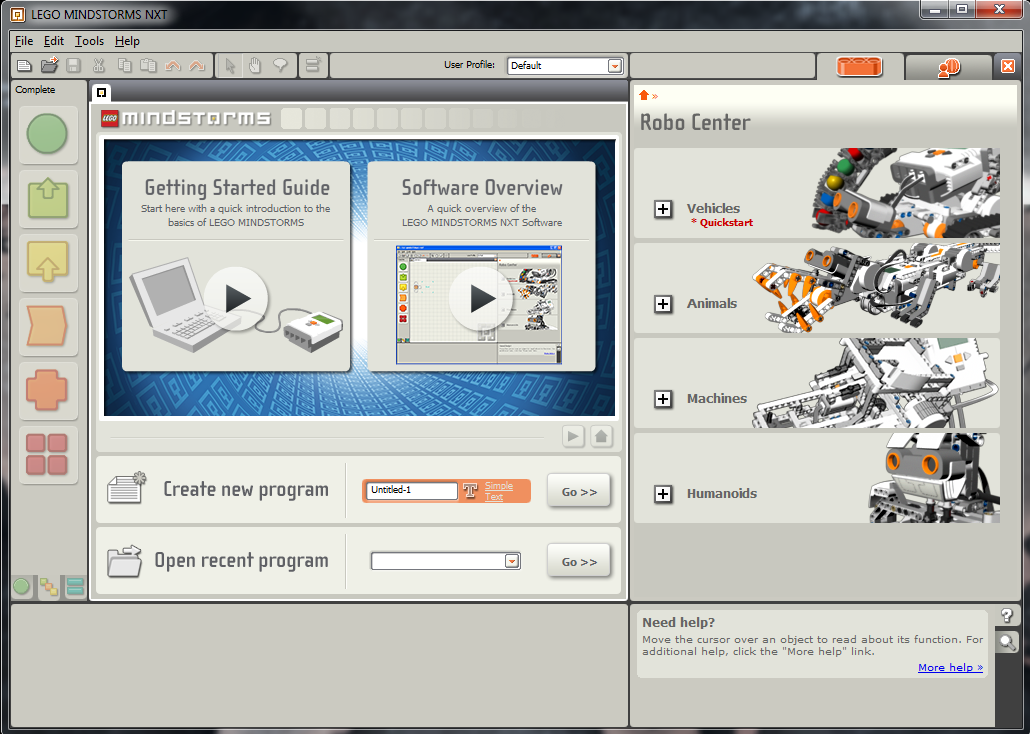
\includegraphics[scale=0.54]{images/Startbildschirm_NXT.png} 
\caption{Der Startbildschirm des LEGO Mindstorms NXT-Programms}
\label{fig:NXT Start}
\end{figure}
Die Abbildung \ref{fig:NXT Start} zeigt den Startbildschirm der Entwicklungsumgebung. Dieser stellt neben zwei Videoanleitungen als Hilfe für Anfänger auch das \emph{Robo Center} zur Verfügung, in dem verschiedene von LEGO vorgeschlagene Roboter-Modelle, die mithilfe des Bausatzes des NXT zusammengesetzt werden können, vorgestellt werden.\\

Sobald eine neue oder bestehende Programmdatei geöffnet wird, können die SuS mithilfe von Blöcken, die unter anderem der Bewegung und Sensorik dienen und dabei einfache Steuerungsmechanismen sowie Elemente der Regelungstechnik zur Verfügung stellen, ihren Roboter programmieren. Hierbei werden Bausteine aus der linken Leiste per Drag-and-Drop auf die karierte Oberfläche gezogen. Es können ineinander geschachtelte Schleifen erstellt werden sowie if-Abfragen mit zwei Fallunterscheidungen. Nahezu beliebig viele Bausteine lassen sich so miteinander kombinieren (Vlg. Abb.\ref{fig:Bsp NXT}).\\

Der Vorteil an dieser Entwicklungsumgebung besteht darin, dass sie von LEGO zur Verfügung gestellt wurde, und somit alle Funktionen von Haus aus mitbringt, die dem NXT-Baustein technisch zur Verfügung stehen. Zudem muss es keine Veränderungen an der Firmware des NXT-Bausteins geben, was eine Zeitersparnis bei der Vorarbeit der SuS mit sich bringt.
\begin{figure}[htbp]
\centering
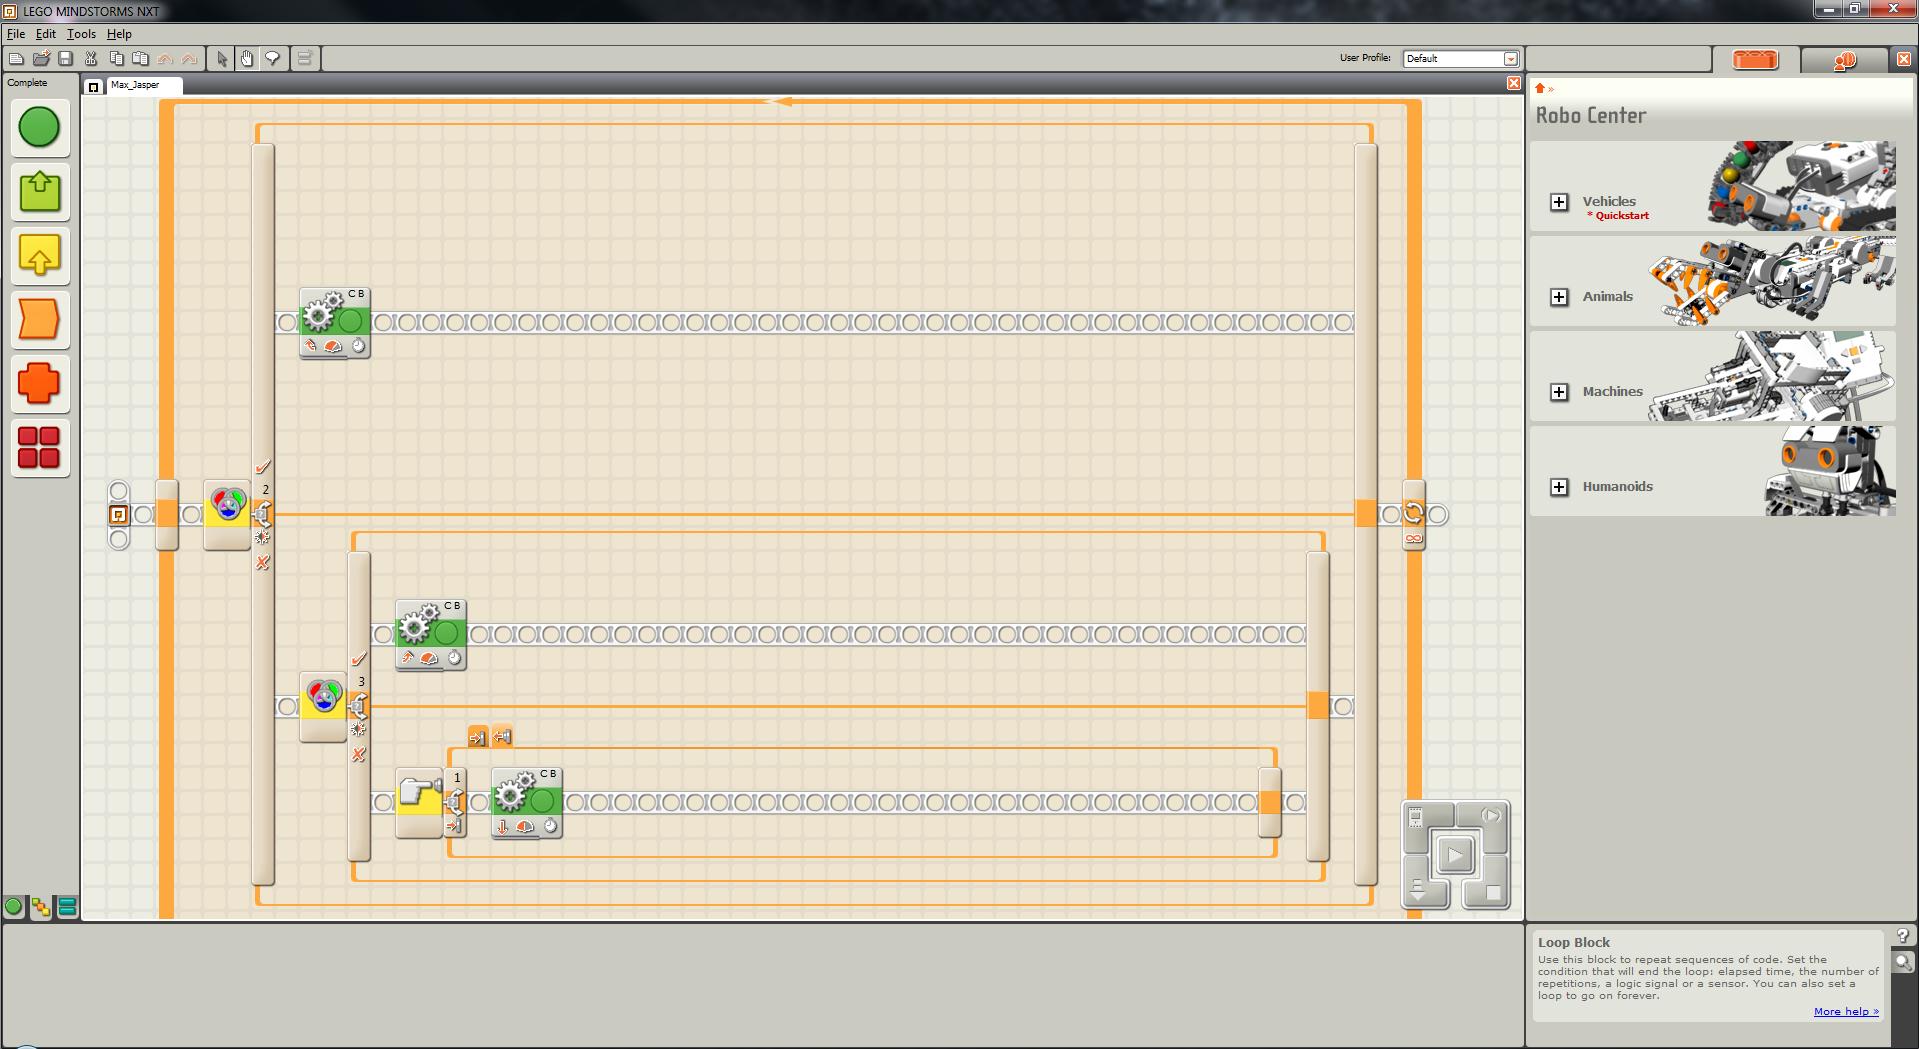
\includegraphics[scale=0.282]{images/Beispielprogramm_NXT.png} 
\caption{Fahren eines Roboters auf einer schwarzen Linie}
\label{fig:Bsp NXT}
\end{figure}

\subsection{Enchanting}
\label{sec:enchanting}
Enchanting ist eine an \emph{Scratch} anknüpfende Entwicklungsumgebung. Wie das in \textbf{\ref{sec:LMNXT}} beschriebene Programm wird auch hier mithilfe von Drag-and-Drop gearbeitet. Da Enchanting keine von LEGO nativ unterstützte Entwicklungsumgebung für NXT Roboter ist, muss hier eine Änderung an der Firmware vorgenommen werden. Hierbei wird die ausgelieferte Standardfirmware mit leJOS (s. \ref{sec:lejos}) ersetzt. Dies sorgt dafür, dass der NXT nun auf die Programmierung mit Java reagiert.\\
\begin{figure}[H]
\centering
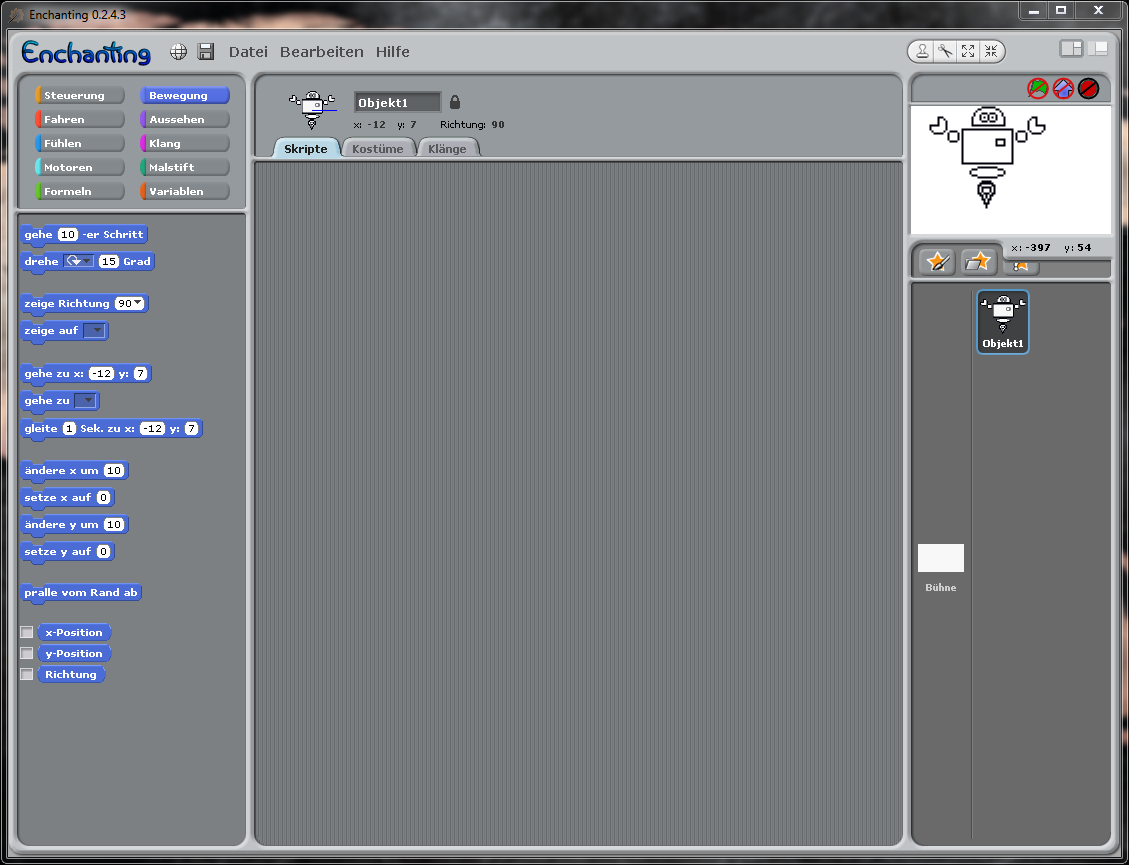
\includegraphics[scale=0.5]{images/Enchanting_Start.png} 
\caption{Der Startbildschirm von Enchanting}
\label{fig:Enchanting Start}
\end{figure}

Wird Enchanting von den SuS geöffnet, erscheint zunächst der Startbildschirm wie in Abb. \ref{fig:Enchanting Start}. Nun kann entweder ein neues Programm erstellt oder ein bestehendes geöffnet werden. Die verschiedenen Programmierelemente werden nach Kategorien in den oberen linken Ecke sortiert aufgeführt. Essentiell dabei sind die Kategorien \emph{Steuerung}, \emph{Fühlen}, \emph{Motoren} und \emph{Formeln}. Die SuS lernen beim Programmieren mit Enchanting, dass sie ihre Motoren und Sensoren zunächst über die verschiedenen Ports referenzieren müssen. Dies geschieht ganz einfach, indem z.B. man einen Motor-Block an einen Port "`setzt"' und ihm einen aussagekräftigen Namen gibt. Auf diese Weise kann nun -- anders als beim LEGO MINDSTORMS NXT-Programm -- bei if-Abfragen und anderen Steuerungselementen mithilfe des Namens auf den Motor oder Sensor zugegriffen werden.\\
\begin{figure}[htbp]
\centering
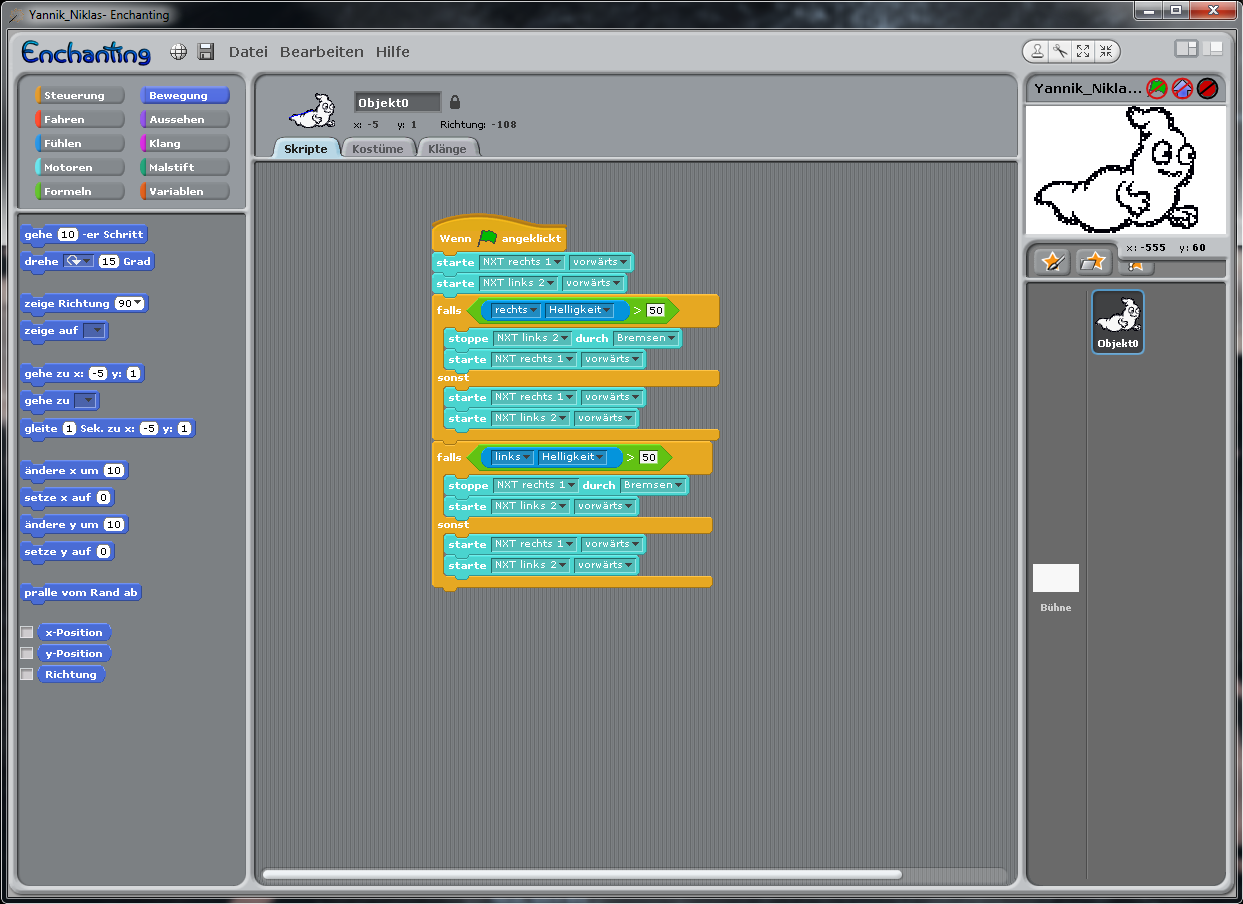
\includegraphics[scale=0.45]{images/Beispielprogramm_Enchanting.png} 
\caption{Beispiel eines Enchanting Programms}
\label{fig:Bsp Enchanting}
\end{figure}
In Abbildung \ref{fig:Bsp Enchanting} ist nun ein simples Programm zum Fahren entlang einer schwarzen Linie mithilfe von zwei Lichtsensoren dargestellt. Hierbei ist zu erkennen, dass die Sensoren in den \texttt{falls...sonst...}-Blöcken mit \texttt{rechts} und \texttt{links}, die Motoren in den türkisfarbenen Elementen mit \texttt{NXT rechts 1} sowie \texttt{NXT links 2} bezeichnet sind. Es kann somit von den SuS direkt gesagt werden, welcher Sensor angesprochen wird, und welcher Motor an welchem Port angeschlossen ist.

\subsection{BlueJ}
\label{sec:bluej}

\par \singlespacing
\section{leJOS}
\label{sec:lejos}
\onehalfspacing
leJOS ist eine kleine Java Virtual Machine und stellt alle Klassen der NXJ API zu Verfügung, mithilfe derer Lego Mindstorms NXT Roboter in Java programmiert werden können \cite{lejos}.


\par \singlespacing
\chapter{Anforderungen an die Neuimplementierung}
\label{chap:anforderungen}
\onehalfspacing
Nicht nur in der Schule, sondern insbesondere in der Wissenschaft spielt Simulation in der Robotik eine wichtige Rolle \cite[S.13]{hertzberg:12}. Die Anforderungen, die an die wissenschaftlichen Simulationsumgebungen der Robotik gestellt werden, fassen \textsc{Hertzberg, Lingemann} und \textsc{Nüchter} wie folgt zusammen:
\begin{itemize}
\item \emph{"`Die Umgebung muss hinreichend gut simuliert sein. Die Simulation einer Flughafenterminalhalle muss zum Beispiel "`zufällig"' umherlaufende Fluggäste mit Gepäck und Transportkarren umfassen.}
\item \emph{Der Roboter in seiner Funktionalität muss hinreichend gut simuliert sein. Das betrifft seine Aktionen wie auch seine Sensorik.}
\item\emph{Relevante Ungenauigkeit technischer Sensoren und Effektoren muss abgebildet werden. Kann zum Beispiel im realen Bild einer Kamera auf dem Roboter ein Orientierungspunkt im Gegenlicht der Fensterfront unsichtbar werden, muss die Simulation diesen Effekt reproduzieren.}
\item \emph{Die "`Wahrheit"' im Simulator ist tabu! Natürlich ist im Simulator der Zustand jedes simulierten Objekts präzise bekannt, einschließlich der Position, Richtung und Geschwindigkeit des Roboters. Die Roboterkontrollsoftware darf hierauf nicht zugreifen, um Information über die Umgebung zu erhalten -- das geht nur über die simulierten Sensoren. (Für die externe Bewertung des Roboterverhaltens ist der Vergleich zwischen der Wahrheit im Simulator und der Information in der Roboterkontrollsoftware aber erlaubt.)}
\item \emph{Der Simulator sollte für den simulierten Roboter die identische Schnittstelle wie der reale Roboter zwischen Roboterkontrollsoftware einerseits und Robotersensorik und -aktuatorik andererseits verwenden; die Roboterkontrollsoftware soll also code-identisch für den realen oder den simulierten Roboter verwendet werden."'} \cite[S.14]{hertzberg:12}
\end{itemize}

In den folgenden beiden Unterkapiteln werden nun die Anforderungen an die Neuimplementierung des Simulator-Prototyps für LEGO Mindstorms NXT Roboter aus Sicht der Schüler und und der Lehrer dargestellt, sowie Parallelen und Unterschiede zu den oben dargestellten herausgearbeitet.

\par \singlespacing
\section{Schülerperspektive}
\label{sec:schüler}
\onehalfspacing
Da es sich bei der Simulationsumgebung um einen Prototypen handelt, der möglicherweise schon ab der fünften, regelmäßig aber ab der siebten Klasse eingesetzt werden soll, steht ein Augenmerk ganz besonders im Fokus: die Einfachheit. Sowohl in der Bedienung des Simulators als auch im Aussehen sollten klare und leicht erkennbare Strukturen vorherrschen.\\

Des weiteren sollte darauf geachtet werden, dass die SuS für die Programmierung des Roboters und die Benutzung des Simulators eine einheitliche Syntax verwenden können. Hierzu muss die Simulationsumgebung genau die Methoden anbieten, die auch bei dem realen Roboter die Steuerung der Motoren und den Zugriff auf Sensordaten ermöglichen. Dies entspricht dem zweiten Aspekt nach \textsc{Hertzberg et al.}, da der simulierte Roboter alle für die Arbeit mit SuS zentralen Funktionen anbieten und sich hinreichend ähnlich wie ein Roboter in der Realwelt verhalten soll. Des weiteren wird hiermit auch der Aspekt der code-identischen Roboterkontrollsoftware erfüllt, da die SuS das selbe Programm für den Simulator, wie auch für den Roboter selbst benutzen können sollten.\\

Ein weiterer Aspekt, den \textsc{Hertzberg et al.} beschreiben sind die Parcours selbst. Diese sollten möglichst realitätsgetreu umgesetzt werden. Das heißt, dass Ausschnitte eines bestehenden realen Wettbewerbsparcours genutzt werden könnten, um für die SuS eine möglichst realitätsnahe Testumgebung anzubieten.\\
\par \singlespacing
\section{Lehrkraft}
\label{sec:lehrkraft}
\par \onehalfspacing
Für Lehrkräfte ist es erfahrungsgemäß wichtig, dass die Simulationsumgebung alle essentiellen Bausteine der objektorientierten Programmierung im Kontext der Lego-Roboter zur Verfügung stellt. Hierzu gehört das Austesten des Fahrens mithilfe einer Schleife, sowie der verschiedenen Sensoren. Hierzu sollte es eine Auswahl an verschiedenen Parcours geben, damit der Fokus bei jedem Parcours auf einer einzigen Sache liegt. Sollen etwa die angebauten Lichtsensoren getestet werden, so bietet es sich an, den Parcours einfach aus einem weißen Hintergrund und einer schwarzen Linie, die entweder senkrecht in der Nähe des Roboters platziert ist, oder als S-Kurve eine Teilstrecke des realen Labyrinths darstellt, bestehen zu lassen.\\
Des weiteren ist es wichtig, dass sich Lehrerinnen und Lehrer schnell in die Simulationsumgebung einarbeiten können, um bei Fragen der SuS sofort Hilfe leisten zu können.

\par \singlespacing
\section{Erweiterbarkeit} \label{sec:erweiterbarkeit}
\onehalfspacing
Die Software sollte ausreichend kommentiert werden, damit auch nach Fertigstellung dieser Masterarbeit weitere Module hinzugefügt werden können. Dies betrifft sowohl die Fähigkeiten der Sensoren, sowie Änderungen, die im Rahmen von Veränderungen der leJOS NXJ API stattfinden, als auch die Möglichkeit, die geschriebene API an die Technologie der LEGO MINDSTORMS EV3, den Nachfolge-Robotern der NXT, anzupassen.
\newpage
\newpage

\par \singlespacing
\chapter{Entwickelte Software}
\onehalfspacing
\par \singlespacing
\section{Prozesse während der Implementation}
\onehalfspacing
Die Entwicklung des Prototyps der Simulationsumgebung umfasste mehrere Schritte, sowie einige Vorarbeit. Diese werden im folgenden Abschnitt nun kurz zusammengefasst.
\par \singlespacing
\subsection{Mock-Ups} 
\onehalfspacing
Um zunächst einen visuellen Grundgedanken festzuhalten und das Ziel der Implementation der vollständigen Simulationssoftware zu erfassen, wurden interaktive Mock-Ups erstellt. Hierzu wurde die Software \emph{Axure RP Pro} benutzt, mit der sich sowohl einfache als auch komplex verschachtelte Mock-Ups erstellen lassen (s. Abb.\ref{fig:axure}).

\begin{figure}[htbp]
\centering
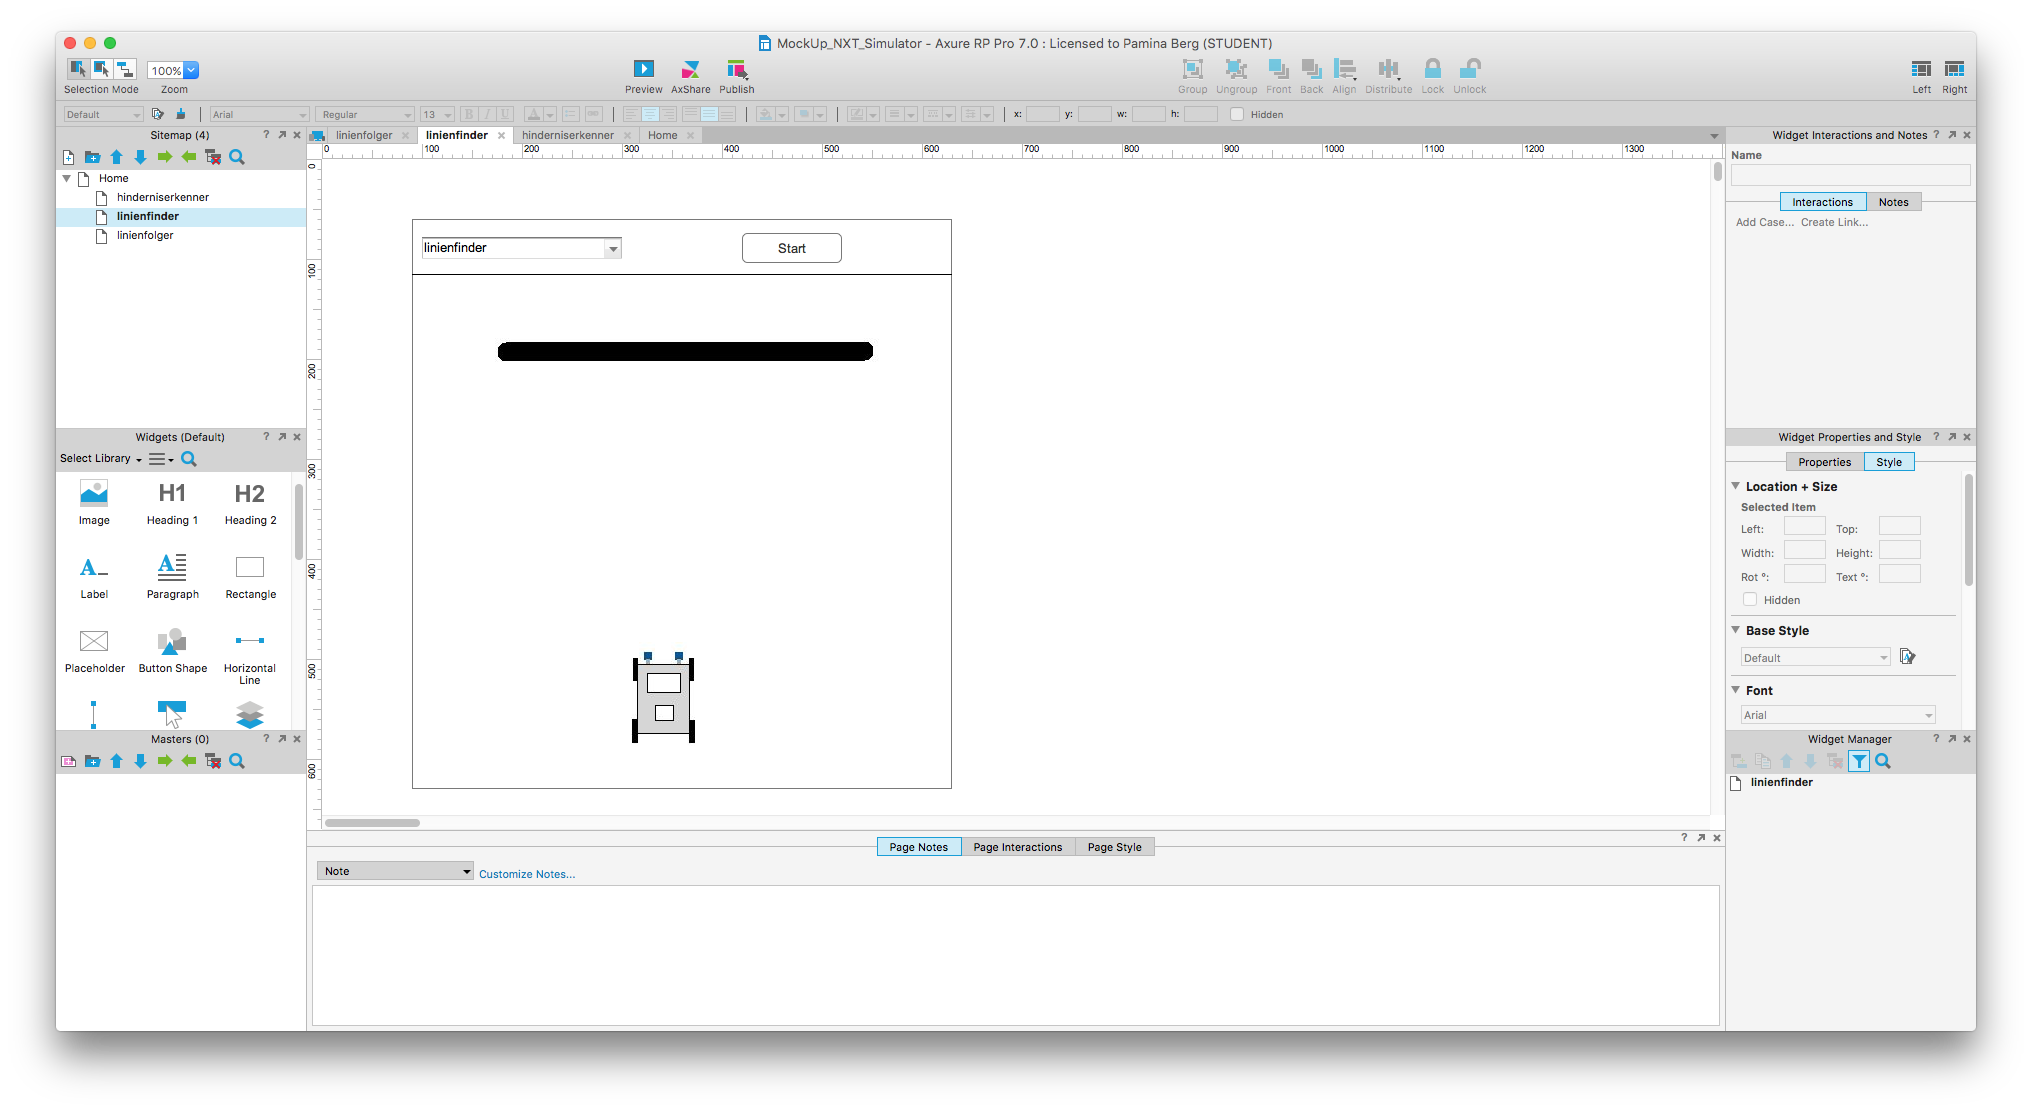
\includegraphics[scale=0.2]{images/axure_mockup.png} 
\caption{Die Bedieneroberfläche von Axure RP Pro}
\label{fig:axure}
\end{figure}

Da die zu schreibende API auch mehrere Sensoren umfasst, sollten die in den Mock-Ups beschriebenen Szenarien den für den Schulkontext erforderlichen Funktionsumfang repräsentieren. Hierzu gehörte das Anhalten auf einer schwarzen Linie wie in Abbildung \ref{fig:linienfinder}, das Fahren entlang einer schwarzen Linie (s. Abb. \ref{fig:linienfolger}) und das Finden und Umfahren eines Hindernisses auf der Fahrbahn (s. Abb. \ref{fig:hinderniserkenner}).

\begin{figure}[htbp]
\centering
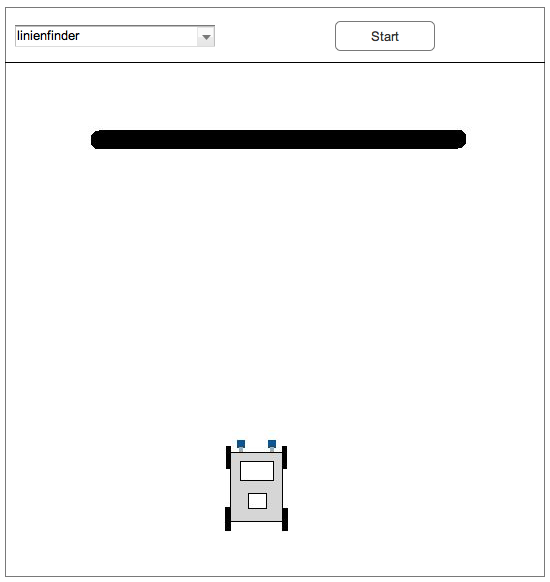
\includegraphics[scale=0.4]{images/mockup_linienfinder.png}
\caption{Anhalten auf einer schwarzen Linie}
\label{fig:linienfinder}
\end{figure}

\begin{figure}[htbp]
\centering
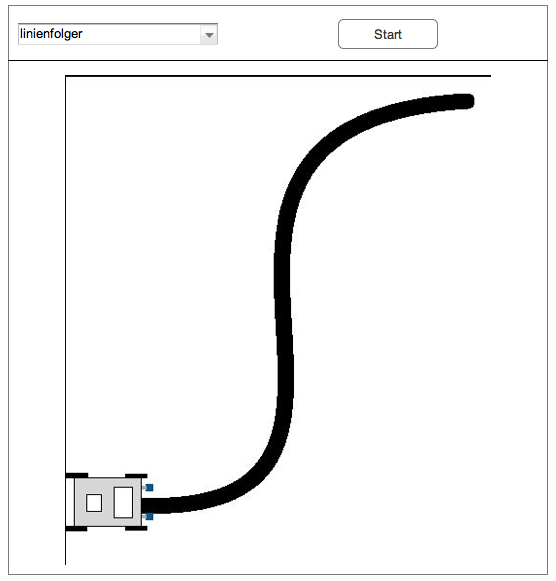
\includegraphics[scale=0.4]{images/mockup_linienfolger.png}
\caption{Fahren einer S-Kurve}
\label{fig:linienfolger}
\end{figure}

\begin{figure}[htbp]
\centering
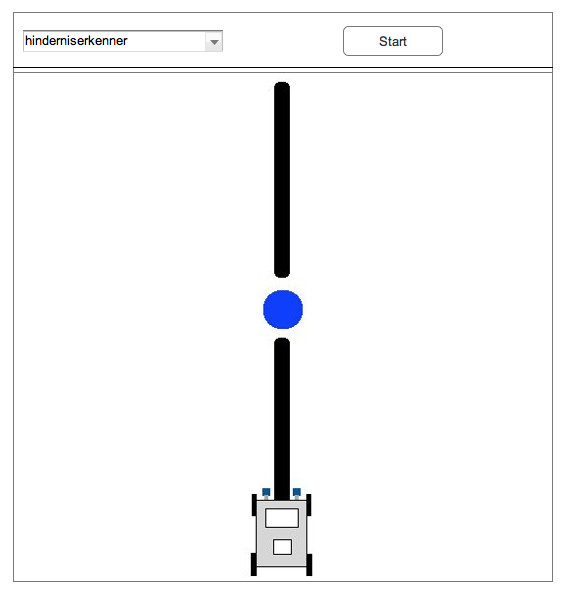
\includegraphics[scale=0.4]{images/mockup_hinderniserkenner.png}
\caption{Erkennen eines Hindernisses auf der Fahrbahn}
\label{fig:hinderniserkenner}
\end{figure}
\par \singlespacing
\subsection{Schritte während der Implementation}
\onehalfspacing
Nach dem Erstellen der Mock-Ups musste nun überlegt werden, inwiefern die Überlegungen umgesetzt werden konnten. Die erste Abstraktion, die während den ersten Implementationsschritten stattgefunden hat, war die Darstellung des Roboters in der Umgebung, so dass dieser einfach als Dreieck implementiert wurde.\\

Außerdem konnte bestehender Code aus anderen Projekten in dieses Projekt importiert werden. So wurde die leJOS API, deren Klassen im Paket der Klassenbibliothek \todo{Kann man das so sagen?} frei verfügbar sind, genutzt, um die Neuimplementation der in \textbf{\ref{sec:API}} beschriebenen Klassen realitätsgetreu miteinander zu verzahnen und die korrekten Beziehungen untereinander zu implementieren.

\par \singlespacing
\subsection{Integration in BlueJ}
\onehalfspacing

\par \singlespacing
\section{Beschreibung der Software}
\onehalfspacing

\par \singlespacing
\section{Softwarearchitektur}
\onehalfspacing 
Die entwickelte Software besteht im derzeitigen Zustand als Prototyp aus insgesamt dreizehn Klassen. Diese lassen sich in zwei Kategorien aufteilen. Zum einen die Klassen, die die API für den Simulator zur Verfügung stellen und die zentralen von leJOS angebotenen Klassen für die NXT-Roboter umfassen, zum anderen die Klassen, die für die Repräsentation der Simulation auf dem Bildschirm zuständig sind.\\

\par \singlespacing
\subsection{Klassen der API}
\label{sec:API}
\onehalfspacing
In diesem Abschnitt werden nun die von leJOS vorgegebenen und an die Implementation des Simulators angepassten Klassen vorgestellt. Hierbei handelt es sich um eine kleine Auswahl der essentiell für den Unterricht erforderlichen Klassen, die im Rahmen dieser Arbeit für den Prototyp angepasst wurden. 
\subsubsection{Motoren}
Zunächst wurde die Klasse \texttt{Motor} implementiert. Diese besteht lediglich aus den Feldern \texttt{A, B} und \texttt{C}, die Exemplare von der Klasse \texttt{NXTRegulatedMotor} darstellen. Ein NXTRegulatedMotor ist ein an einen Motorport angeschlossener NXT-Motor. Diese Klasse bietet die Methoden \texttt{forward(), backward()} und \texttt{stop()} an, die die essentiellen Methoden für die Bewegung des Roboters darstellen. Ein an einen Motorport angeschlossener Motor wird über den Befehl \texttt{Motor.[port].[Methode]} angesteuert. Die Klasse \texttt{MotorPort} ist in diesem Projekt eine verkleinerte Version der gleichen Klasse aus der leJOS API.
\subsubsection{Licht- und Farbsensoren}
Die Lichtsensoren sind zwei von der leJOS-API vorgegebene Exemplare der Klasse \texttt{LightSensor}. Diese sind im Prototyp der Simulation jeweils im Abstand von fünf Pixeln links und rechts von der Spitze des Roboter-Dreiecks angebracht. Da es sich bei der Implementation um einen Prototyp handelt, gibt es noch keine optische Repräsentation der beiden Sensoren am Roboter.\\

Die Klasse \texttt{Roboter} enthält die Methoden zur Abfrage der Positionen der Sensoren im Bezug auf die x- und y-Achse: \texttt{gibXLichtRechts()}, \texttt{gibYLichtRechts()},\\
\texttt{gibXLichtLinks()} und \texttt{gibYLichtsLinks()}. Diese werden benötigt, um das Auslesen des Farbwerts des Pixels unter dem jeweiligen Sensor zu ermöglichen. Die eigentliche Abfrage des Helligkeitswertes passiert jedoch am Parcours-Objekt. In diesem steht die Methode \texttt{gibHelligkeitswert(int x, int y)} zu Verfügung, die auf das Bilddaten-Array zugreift.\\

Die Implementation der Farbsensoren ist im Simulator code-identisch, daher kann in dieser Ausarbeitung auf eine explizite Beschreibung verzichtet werden.
\subsubsection{Ultraschall- und Berührungssensor}
Der Berührungssensor, oder wie von leJOS TouchSensor genannt, ist im Simulator an der vordersten Spitze des Roboter-Objekts platziert. Da Hindernisse im Simulator schwerlich als mehrdimensionale Objekte dargestellt werden können, wird in diesem Prototyp zunächst mit einer Farbunterscheidung gearbeitet. Dies funktioniert wiederum über den Helligkeitswert des Pixels, der sich gerade unter der Spitze des Roboter-Objekts befindet.\\

Für die Implementation des Ultraschallsensors wird eine Implementation des Hindernisses als Objekt auf dem Parcours benötigt. Dies ist nicht essentiell für die Implementation eine ersten Prototypen des Simulators, da die für SuS relevanten Aufgaben auch mit einem Berührungssensor gelöst werden können. Daher verzichtet dieser Prototyp zunächst auf die Implementation eines Ultraschallsensors.
\subsubsection{Sensorports}
Jeder der eben genannten Sensoren ist an einen so genannten Sensorport angeschlossen. Die Klasse \texttt{SensorPort} enthält Felder, die die einzelnen Ports darstellen. Ein Exemplar einer Sensoren-Klasse wird bei der Initialisierung stets an einen Sensorport gekoppelt. 

\par \singlespacing
\subsection{Die Simulationsumgebung}
\onehalfspacing
Nun zu einer Beschreibung der Struktur der Simulationsumgebung selbst. Hierzu gehört die grafische Repräsentation des Parcours, des Roboters, der Auswahldialog für den Parcours, sowie die Leinwand, auf der der simulierte Roboter fahren soll.
\subsubsection{Simulator}
Der Simulator erzeugt beim Ausführen zunächst einen \texttt{BildEinleser}. Dieser lässt den Benutzer in einem Dialogfenster eine .gif-Datei als Parcours auswählen. Das ausgewählte Bild wird dann "`eingelesen"' und die einzelnen Bildpunkte in einem short-Array gespeichert.
\subsubsection{Bildeinleser}
Die Klasse \texttt{BildEinleser} besitzt keinen Konstruktor, da diese nur als Hilfsklasse bestimmte Methoden zur Verfügung stellen muss. Durch den Aufruf der Methode\\
\texttt{liesBilddaten()} eines Bildeinlesers wird ein JFileChooser erzeugt, mithilfe dessen der Benutzer eine Bilddatei auswählen kann, auf der der Roboter simuliert werden soll. Danach wird das Bild so umgewandelt, dass ein Array aus Bildpunkten entsteht.
%In dem dieser Arbeit vorangegangenen Studium wurde bereits mit Projekten gearbeitet, in denen Bilddateien eingelesen und benutzt wurden, daher wurde diese Klasse aus einem alten Projekt importiert.\\
\subsubsection{Parcours}
Die Klasse Parcours ist dafür zuständig, dass eine Leinwand erzeugt und dann das Bild des Parcours angezeigt wird. Dies geschieht durch die Speicherung der Bilddaten des Bildes in der Feldvariable \texttt{{\_}bilddaten}, die dann an die Leinwand weitergegeben werden.\\

Gleichzeitig ist sie die Schnittstelle zwischen Simulator und den API-Klassen, da sie dafür zuständig ist, Informationen über den Parcours an die Sensoren weiterzuleiten. Insbesondere die Abfrage des Helligkeitswerts eines Pixels aus dem Array ist in dieser Klasse implementiert.
\subsubsection{Leinwand}

\newpage
\chapter{Zusammenfassung und Ausblick}

\newpage
\begin{thebibliography}{ABCD}

\renewcommand{\refname}{\normalsize Literaturverzeichnis}

\bibitem[Abe01]{abend:01}
Michael Abend. "'Robotik und Sensorik. Darstellungsschwerpunkt: Selbständige Entwicklung "`unscharfer"' Algorithmen zur räumlichen Orientierung (unter Verwendung des LEGO-Mindstorms-Systems)", \emph{Schriftliche Prüfungsarbeit zur zweiten Staatsprüfung für das Amt des Studienrats}, Berlin, 2001

\bibitem[Her12]{hertzberg:12}
Joachim Hertzberg, Kai Lingemann, Andreas Nüchter. \emph{Mobile Roboter. Eine Einführung aus Sicht der Informatik}, Springer-Verlag Berlin Heidelberg, 2012

\bibitem[Hub07]{hubwieser:07}
Peter Hubwieser. \emph{Didaktik der Informatik}, 3. Auflage, Springer-Verlag Berlin Heidelberg, 2007

\bibitem[Lego]{lego}
o.V. URL: \url{http://www.lego.com/en-us/mindstorms/history}, Abgerufen am 06.11.2015, LEGO, 2015

\bibitem[leJOS]{lejos}
o.V. URL: \url{http://www.lejos.org/nxj.php}, Abgerufen am 14.12.2015, leJOS Java for Lego Mindstorms, 2015

\bibitem[Nie99]{nievergelt:99}
Jürg Nievergelt. \emph{"Roboter programmieren" - ein Kinderspiel. Bewegt sich auch etwas in der Allgemeinbildung?}, Informatik-Spektrum 22:5, S. 364--375, 1999

\bibitem[Rol14]{rolling:14}
Mark Rollins. \emph{Beginning LEGO MINDSTORMS EV3}, Apress, Berkeley, CA, 2014

\bibitem[Sch04]{schreiber:04}
Rafael Schreiber. "Der Einsatz von LEGO-Mindstorms im Informatikunterricht der 11. Klasse der Leonard-Bernstein-Oberschule. Sicherung und Transfer grundlegender algorithmischer Strukturen in NQC.", \emph{Schriftliche Prüfungsarbeit im Rahmen der zweiten Staatsprüfung für das Amt des Studienrats}, Berlin, 2004

\bibitem[Sto01]{stolt:01}
Matthias Stolt. "Roboter im Informatikunterricht", 2001

\bibitem[Wag05]{wagner:05}
Oliver Wagner. "LEGO Roboter im Informatikunterricht. Eine Untersuchung zum Einsatz des LEGO-Mindstorms-Systems zur Steigerung des Kooperationsvermögens im Informatikunterricht eines Grundkurses (12. Jahrgang, 2. Lernjahr) der Otto-Nagel-Oberschule (Gymnasium)", \emph{Schriftliche Prüfungsarbeit im Rahmen der zweiten Staatsprüfung für das Amt des Studienrats}, Berlin, 2005

\end{thebibliography}
\newpage
\thispagestyle{empty}
\vspace*{\fill}
"Hiermit versichere ich, dass ich die Arbeit selbstständig verfasst und keine anderen als die angegebenen Hilfsmittel – insbesondere keine im Quellenverzeichnis nicht benannten Internet-Quellen – benutzt habe, die Arbeit vorher nicht in einem anderen Prüfungsverfahren eingereicht habe und die eingereichte schriftliche Fassung der auf dem elektronischen Speichermedium entspricht."\\

Hamburg, \today \hspace*{\fill} \dots \dots \dots \dots \dots \dots \dots\\
\hspace*{\fill} Pamina Maria Berg $\,$
\end{document}